\documentclass[11pt,a4paper]{report}
\usepackage[margin=24mm]{geometry}
\usepackage[T1]{fontenc}
\usepackage{lmodern,microtype,amsmath,amssymb,booktabs,graphicx,subcaption,float,hyperref,xcolor}
\newcommand{\SI}[2]{#1\,\ensuremath{\mathrm{#2}}}
\newcommand{\giga}{G}
\newcommand{\hertz}{Hz}
\newcommand{\metre}{m}
\newcommand{\degree}{^\circ}
\hypersetup{colorlinks=true,linkcolor=blue!45!black,urlcolor=blue!45!black}
\graphicspath{{../public_results/}}
\setcounter{secnumdepth}{2}
\title{Panel Deformation and Monopulse Azimuth Error in a Synthetic Cylindrical Array\\\large Public Modeling and Simulation Report}
\author{Engineering portfolio study}
\date{24 October 2026 \quad Public portfolio version 1.0}
\begin{document}
\maketitle
\begin{abstract}
A frequency-dependent phase centre on a flexible radial panel converts correlated mechanical displacement into changes in array phase, beam pointing, and monopulse estimation. This report documents a reproducible public C-band model with 60 equally spaced cylinder columns, a contiguous 20-column active sector, and 16 elements per column. It distinguishes the peak direction of the sum response from the angle inferred using a nominal difference-to-sum calibration. In 500 synthetic realizations at \SI{5.8}{\giga\hertz}, the deformed-stack scenario gives \SI{0.085448}{\degree} beam-peak shift RMSE and \SI{0.084084}{\degree} monopulse angle-error RMSE. These numerical settings and results belong to this public simulation; they are not dimensions or measurements of the underlying engineering system. The mechanical team's assessment of the modeling approach and the project assessment of acceptable modeled error are reported context, not public acceptance criteria. The mechanical response has not been validated against a complete structural model, and neither mechanical nor RF response has been measured on hardware.
\end{abstract}
\tableofcontents
\chapter{Problem and scope}
A beamformer compensates the nominal phase of each receive element. Correlated panel movement changes its effective position while the stored weights remain tied to the nominal array. Both the maximum of the sum beam and the inverse of the monopulse ratio can move. Their errors need separate definitions: a similar RMSE over many realizations does not establish equal error in an individual realization. This report adapts the scientific organization of the source project report while replacing its configuration and results with the independently runnable public implementation. No source organization, personnel, hardware dimensions, internal acceptance limit, or original measurement is disclosed.

The public code contains a MATLAB rewrite and a Python implementation. Python generated the numerical plots and CSVs used here. The MATLAB version has not been run in a MATLAB environment for this public release; exact Monte Carlo traces are not expected to match across generators. Results characterize model behavior under stated assumptions rather than measured antenna performance.

\chapter{Array geometry and receive model}
\section{Public geometric configuration}
At reference frequency $f_h=\SI{5.8}{\giga\hertz}$, $\lambda_\mathrm{ref}=c/f_h=\SI{0.051688}{\metre}$. The public vertical spacing and circumferential chord pitch are $d=\lambda_\mathrm{ref}/2=\SI{0.025844}{\metre}$. With $N=60$ columns, the radius is
\begin{equation}R=\frac{d}{2\sin(\pi/N)}\simeq\SI{0.246907}{\metre}.\end{equation}
The nominal active aperture comprises 20 consecutive columns centred on the boresight and 16 rows, or 320 active phase centres. The full cylinder has an angular column pitch of \SI{6}{\degree}; the active centres span \SI{-57}{\degree} to \SI{57}{\degree}. The row-centre span is $15d\simeq\SI{0.387663}{\metre}$. The physical extent of a flexible sheet away from its root is a schematic drawing parameter and is not inferred from these phase-centre coordinates.
\begin{figure}[htbp]\centering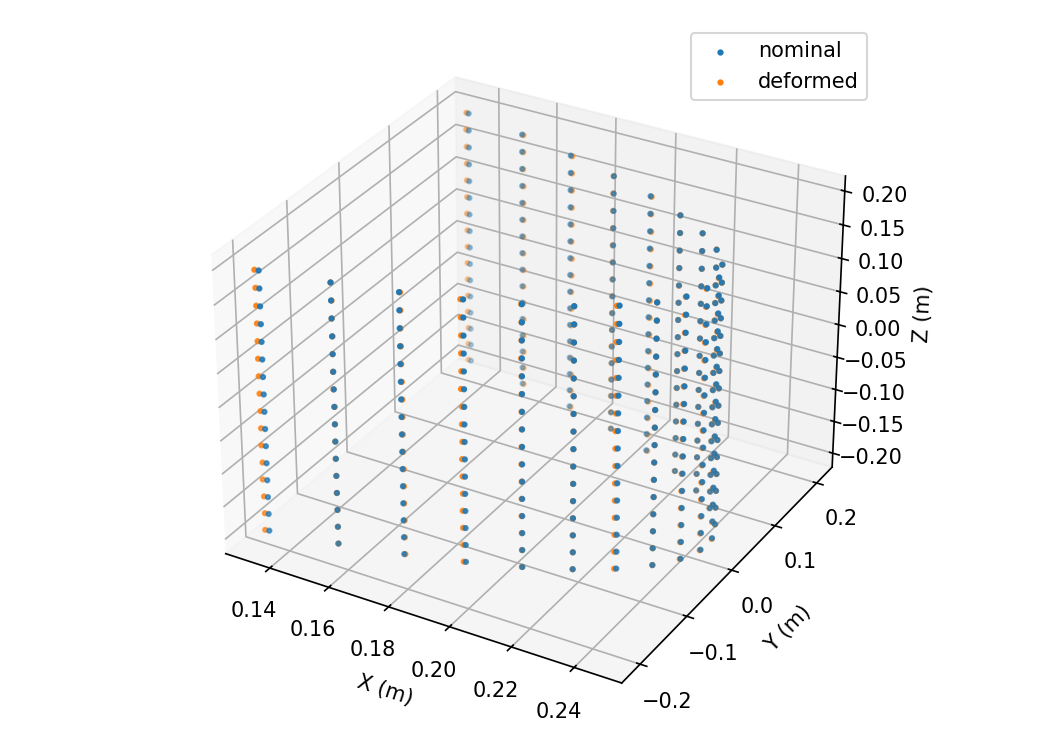
\includegraphics[width=.76\textwidth]{02_geometry.png}\caption{Nominal and one deformed realization of active element phase-centre positions. Physical displacements are small on this axis scale.}\end{figure}
\section{Signal response and channel architecture}
For target azimuth $\alpha$ and elevation $\epsilon$, the unit arrival vector is $\mathbf u=(\cos\epsilon\cos\alpha,\cos\epsilon\sin\alpha,\sin\epsilon)^T$. A phase centre $\mathbf r_n$ contributes $a_n=\exp(jk\mathbf r_n\cdot\mathbf u)$, with $k=2\pi f/c$. The computed sum and difference are $\Sigma=\sum_n w_{\Sigma,n}a_n$ and $\Delta=\sum_n w_{\Delta,n}a_n$. The public baseline assumes isotropic elements and omits mutual coupling, receiver noise, channel gain/phase errors, and rotation of element normals.

A Hamming window weights 20 azimuth columns; a Taylor window weights 16 rows. Each row supplies left- and right-half channels, yielding 32 subarray channels. The difference channel changes sign across the two halves. Scenario A uses a single elevation beam with analog setting matched to that beam; B applies a nominal stack with a separate analog elevation setting. C and D apply the same respective weights to displaced coordinates. The response-surface display takes a pointwise maximum over five elevation settings for the stack; that display operation is not a separate physical receiver model.
\begin{figure}[htbp]\centering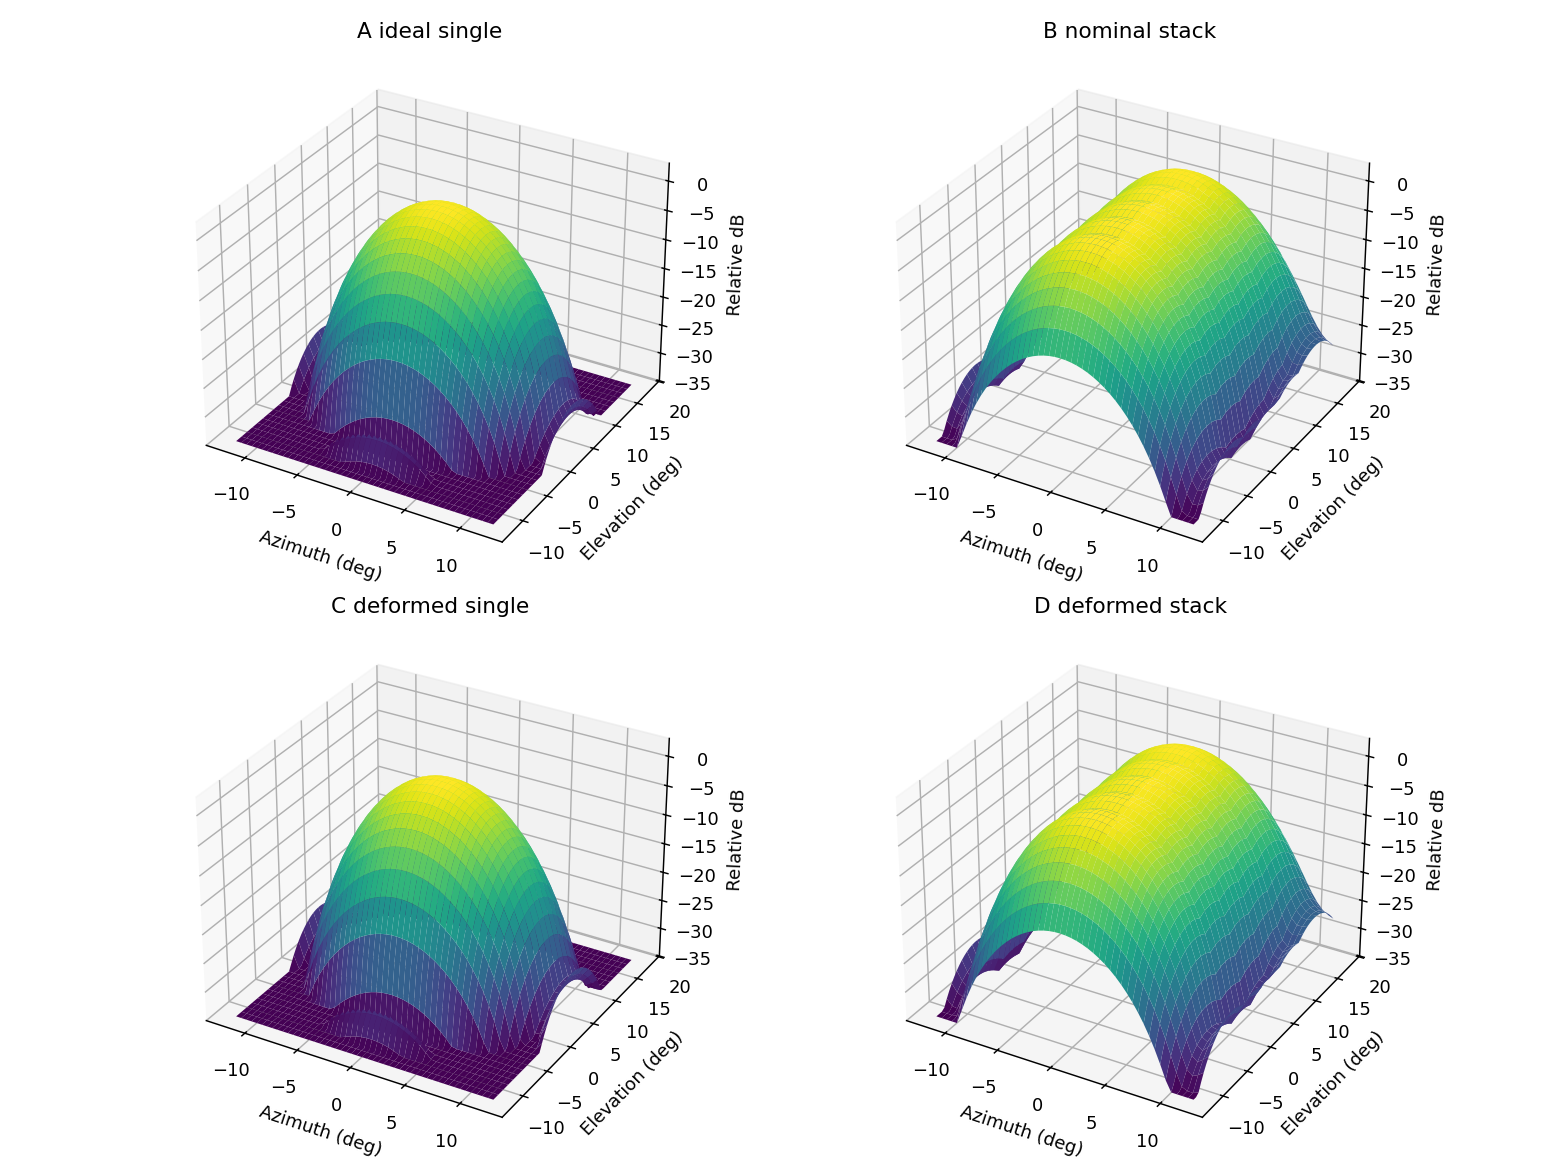
\includegraphics[width=.78\textwidth]{10_receive_patterns_3d.png}\caption{Calculated receive-response surfaces for the four public scenarios, normalized to the nominal B peak. The plotted stack envelope is a display summary.}\end{figure}

\chapter{Correlated panel displacement}
\section{Random field and frequency dependence}
The active sector is an open arc. Panel correlation is $K_{ij}=\exp[-|s_i-s_j|/\ell]$, with $s_i=R\phi_i$ and $\ell$ chosen so neighbouring panels have correlation $\rho_p=0.35$. First and last active panels are not neighbours. For a panel vector $\mathbf p\sim\mathcal N(0,K)$ and independent unit-normal element residual $\eta_n$,
\begin{equation}q_n=\sqrt{\rho_w}\,p_{j(n)}+\sqrt{1-\rho_w}\,\eta_n,\qquad\rho_w=0.995.\end{equation}
At the reference tip, the tangential standard deviation is $\sigma_t=0.02\lambda_\mathrm{ref}$. The nominal mean is zero. The radial and vertical components share this random field, at ratios $10^{-4}$ and $0.02$ respectively; they are not independent Gaussian fields.

For $f_l=\SI{5.2}{\giga\hertz}$ and $f_h=\SI{5.8}{\giga\hertz}$, the normalized effective position is $\xi=[(f-f_l)/(f_h-f_l)]^{p}$, with $p=1$ by default. The uniform-load cantilever-inspired normalized bending gain used in the code is
\begin{equation}g(\xi)=\frac{\xi^2(6-4\xi+\xi^2)}{3},\qquad g(0)=0,\quad g(1)=1.\end{equation}
Thus $d_{t,n}=g(\xi)\lambda_\mathrm{ref}(\mu_t+\sigma_t^*q_n)$, where $\mu_t=0$ and $\sigma_t^*=0.02$ are dimensionless tip settings. The alternate tip-force shape is available in code but is not the baseline. Cartesian displacement follows $\delta\mathbf r_n=(-\sin\phi_n d_t+\cos\phi_n d_r,\,\cos\phi_n d_t+\sin\phi_n d_r,\,d_z)^T$. The phase perturbation at fixed arrival direction is $\delta\psi_n=k\delta\mathbf r_n\cdot\mathbf u$.

This is a parameterized random-displacement model, not a load-to-deflection finite-element prediction. The team's judgment that it was sufficient for the project's random-motion analysis does not constitute independent structural validation. The separate portfolio illustration enlarges sheet bending 30-fold only in its geometry view; RF computations here always use the modeled displacement without that enlargement.
\begin{figure}[htbp]\centering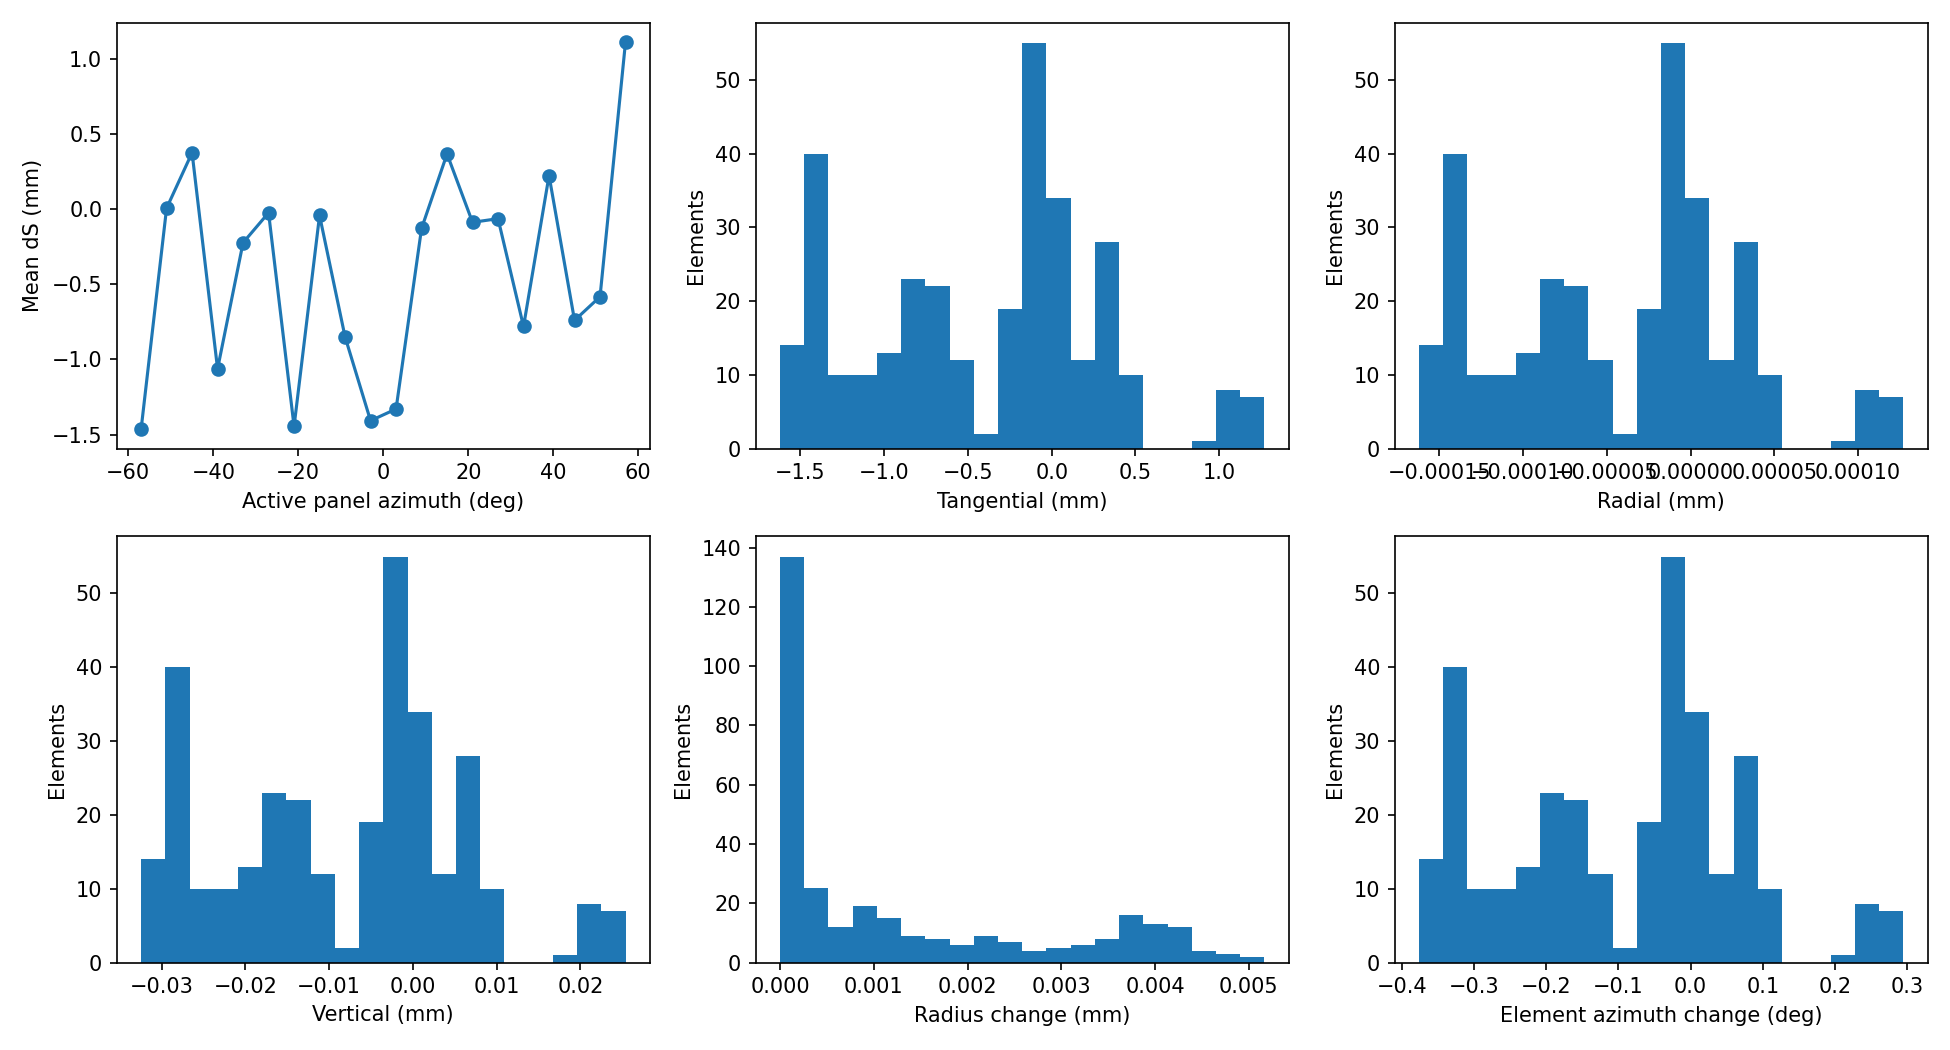
\includegraphics[width=.85\textwidth]{03_displacement.png}\caption{One random field: mean tangential movement across active panels and element-level tangential, radial, vertical, radius-change, and azimuth-change distributions.}\end{figure}
\begin{figure}[htbp]\centering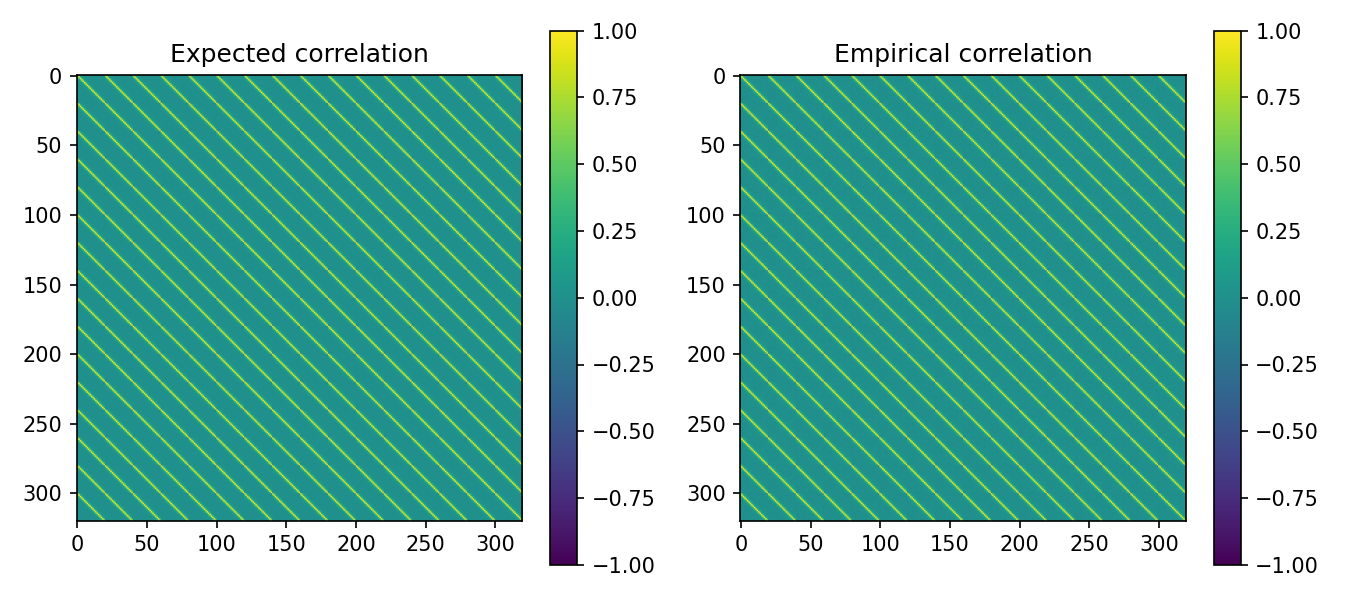
\includegraphics[width=.75\textwidth]{01_generator_validation.png}\caption{Expected and empirical correlation matrices from 10,000 draws at the upper-band endpoint. This is a generator check, not physical validation.}\end{figure}

\chapter{Angle estimation and scenarios}
The public steering azimuth is zero; the example target is at \SI{1}{\degree} azimuth and \SI{4}{\degree} elevation. With nominal B weights and nominal coordinates, the calibration map is $m_0(\alpha)=\operatorname{Im}(\Delta/\Sigma)$. The implementation finds a monotone valid interval around boresight where $|\Sigma|$ exceeds 10\% of its nominal maximum; an estimate outside its ratio range is NaN, not an extrapolated angle. For each scenario, the measured ratio is inverted against \emph{the same nominal B calibration}. Consequently, a displaced response can produce bias even when the sum-beam shape changes little.

The reference beam peak is nominal B at the beam elevation. For each realization, beam error is $e_b=\alpha_{\mathrm{peak}}-\alpha_{\mathrm{peak},B}$; angle-estimation error is $e_m=\widehat\alpha-\alpha_\mathrm{true}$. The program uses a coarse peak grid followed by bounded local optimization. It stores invalid or boundary cases separately. The statistics below are conditional on finite estimates; each CSV records its invalid count.
\begin{figure}[htbp]\centering\begin{subfigure}{.49\textwidth}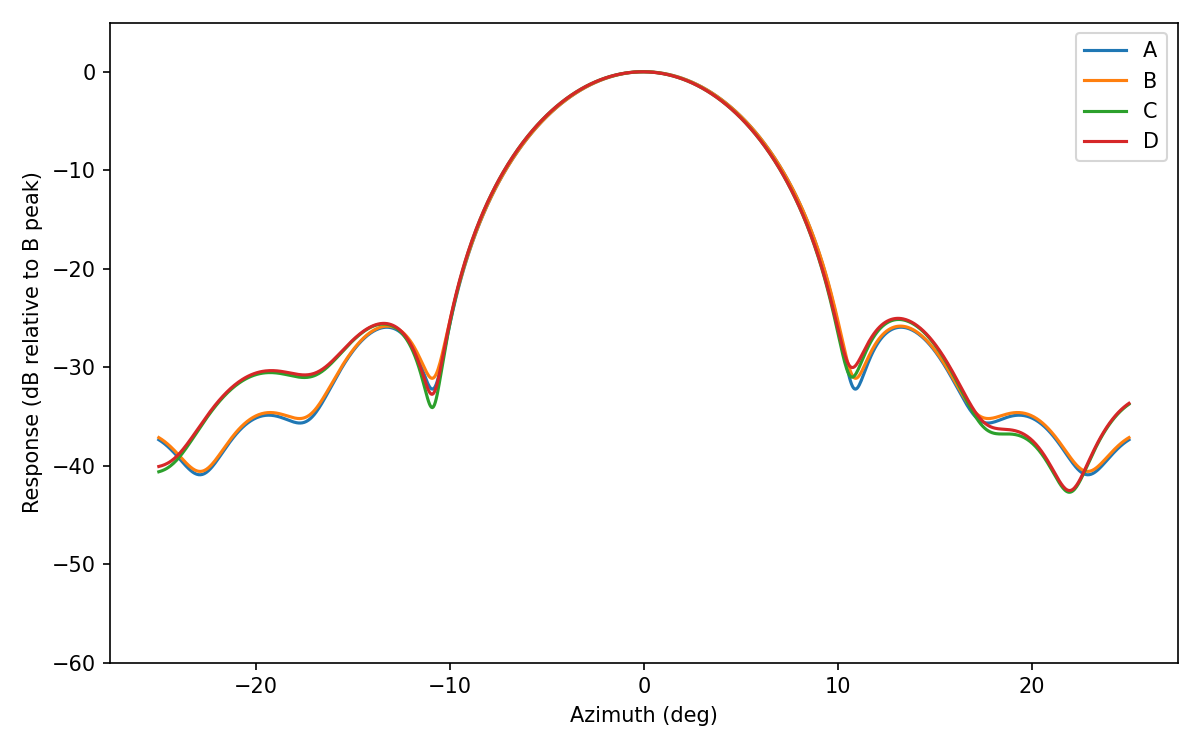
\includegraphics[width=\linewidth]{04_pattern.png}\caption{Sum-beam cut.}\end{subfigure}\hfill\begin{subfigure}{.49\textwidth}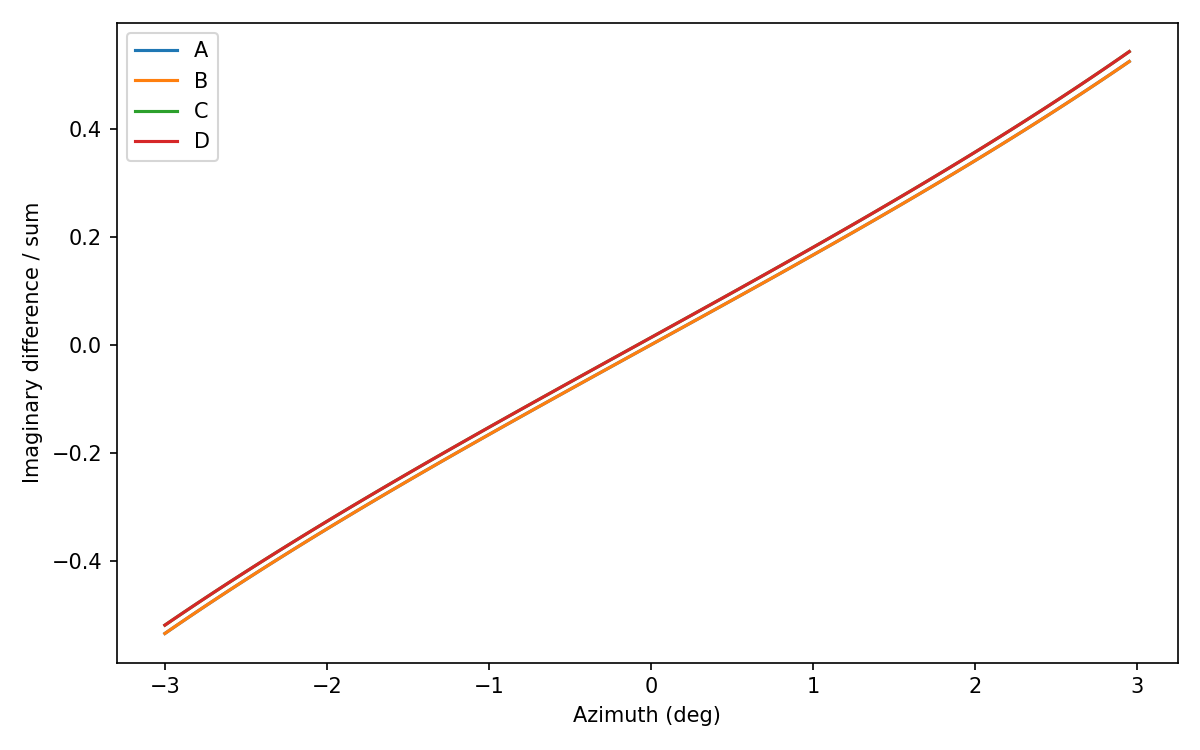
\includegraphics[width=\linewidth]{05_monopulse_curve.png}\caption{Imaginary difference/sum.}\end{subfigure}\caption{One realization and nominal references A--D. Patterns use the B peak as reference; the ratio is shown only on the valid calibration domain.}\end{figure}

\chapter{Numerical experiment and findings}
\section{Monte Carlo definitions}
The Python baseline uses seed 3719 and 500 independently drawn mechanical fields. For finite errors $e_i$, $\mathrm{bias}=n^{-1}\sum_i e_i$, $\mathrm{RMSE}=\sqrt{n^{-1}\sum_i e_i^2}$, and reported standard deviation uses the population convention. The displayed 95\% interval for the \emph{mean} is the normal approximation $\bar e\pm1.96s/\sqrt n$ with sample $s$; it is not a 95\% interval for individual error and should not be used as a system acceptance bound.

\begin{table}[htbp]\centering\caption{Baseline public results at \SI{5.8}{\giga\hertz}; 500 realizations. Values are rounded from \texttt{scenario\_summary.csv}.}\small\begin{tabular}{lrrrr}\toprule
Scenario & Beam bias & Beam RMSE & Angle bias & Angle RMSE\\\midrule
A ideal single & 0.000000 & 0.000000 & 0.000025 & 0.000025\\
B nominal stack & 0 & 0 & 0 & 0\\
C deformed single & 0.008251 & 0.085481 & -0.006905 & 0.084089\\
D deformed stack & 0.008242 & 0.085448 & -0.006924 & 0.084084\\\bottomrule
\end{tabular}\end{table}

\begin{figure}[htbp]\centering\begin{subfigure}{.48\textwidth}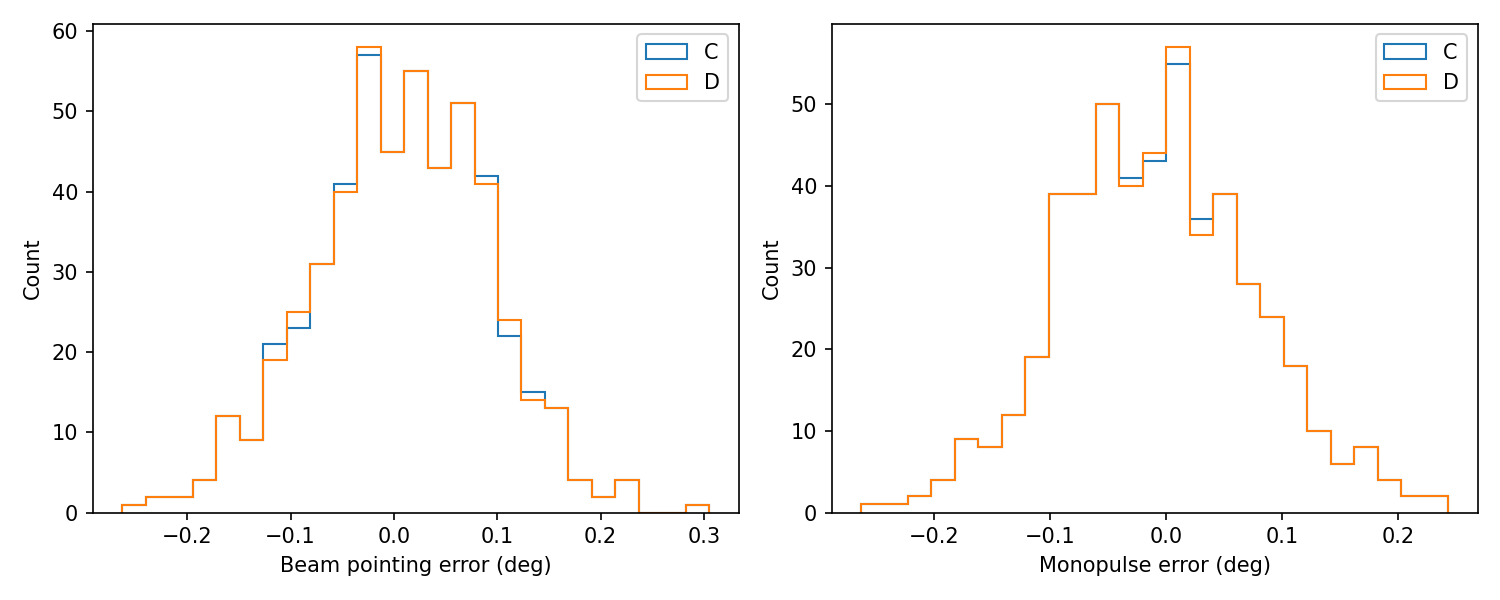
\includegraphics[width=\linewidth]{06_errors.png}\caption{Error distributions.}\end{subfigure}\hfill\begin{subfigure}{.48\textwidth}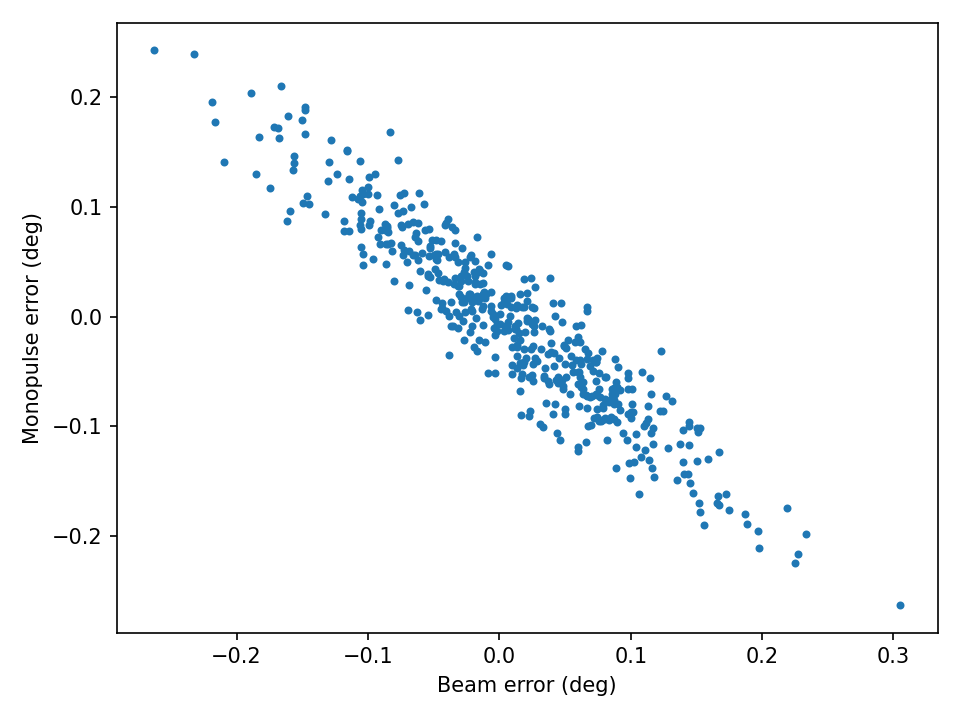
\includegraphics[width=\linewidth]{07_error_relationship.png}\caption{Paired errors for D.}\end{subfigure}\caption{Beam and monopulse estimates respond to the same realization, but remain distinct quantities.}\end{figure}
\begin{figure}[htbp]\centering\begin{subfigure}{.48\textwidth}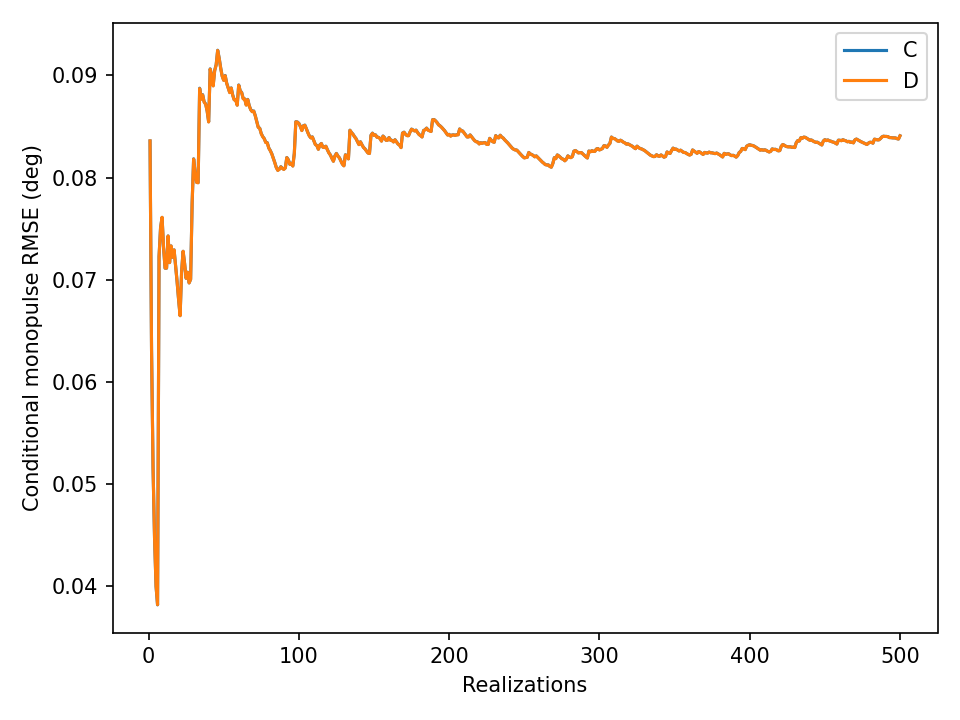
\includegraphics[width=\linewidth]{08_convergence.png}\caption{Running conditional RMSE.}\end{subfigure}\hfill\begin{subfigure}{.48\textwidth}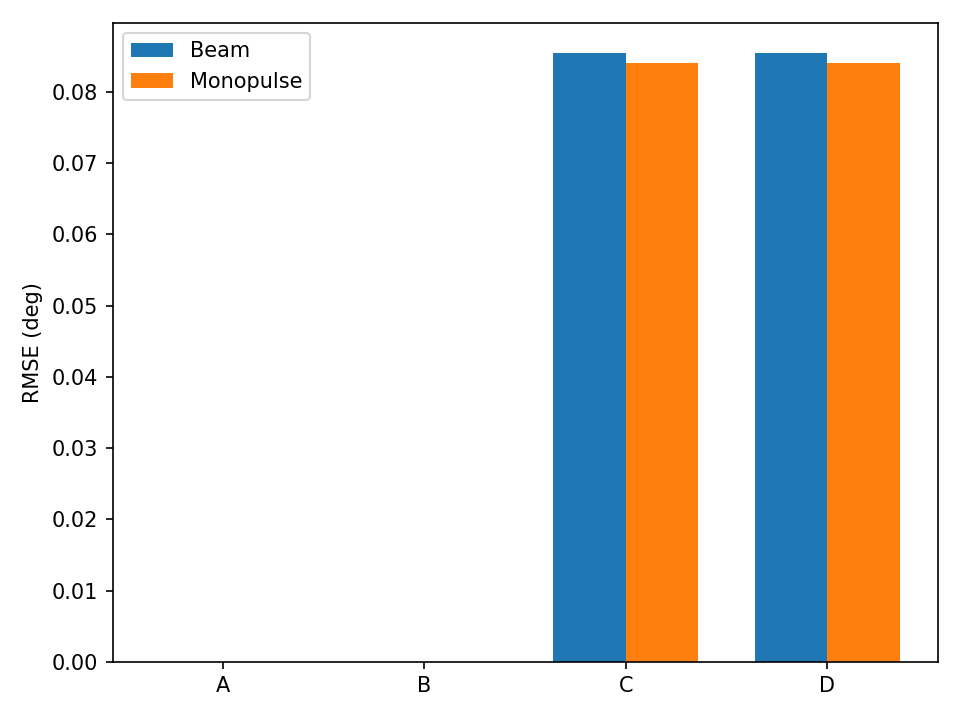
\includegraphics[width=\linewidth]{09_scenarios.png}\caption{Scenario RMSE.}\end{subfigure}\caption{Sampling trajectory and four-scenario comparison. A running curve is a diagnostic, not proof of convergence under every model setting.}\end{figure}

\section{Band and sensitivity interpretation}
At the lower frequency endpoint the modeled phase centre is at the fixed root and $g(0)=0$, so deformation-induced errors vanish in this model. For D, the monopulse RMSE across the five frequencies 5.2, 5.35, 5.5, 5.65, and 5.8 GHz is approximately 0, 0.008862, 0.029767, 0.056155, and 0.084084 degrees. The progression combines phase-centre gain and RF frequency; it cannot be read as a universal scaling law for other antennas. The CSV sweeps vary model parameters separately. For example, larger prescribed tip spread increases modeled angle error, while the public results alone do not establish a mechanical tolerance or a probability of meeting an undisclosed requirement.
\begin{figure}[htbp]\centering\begin{subfigure}{.48\textwidth}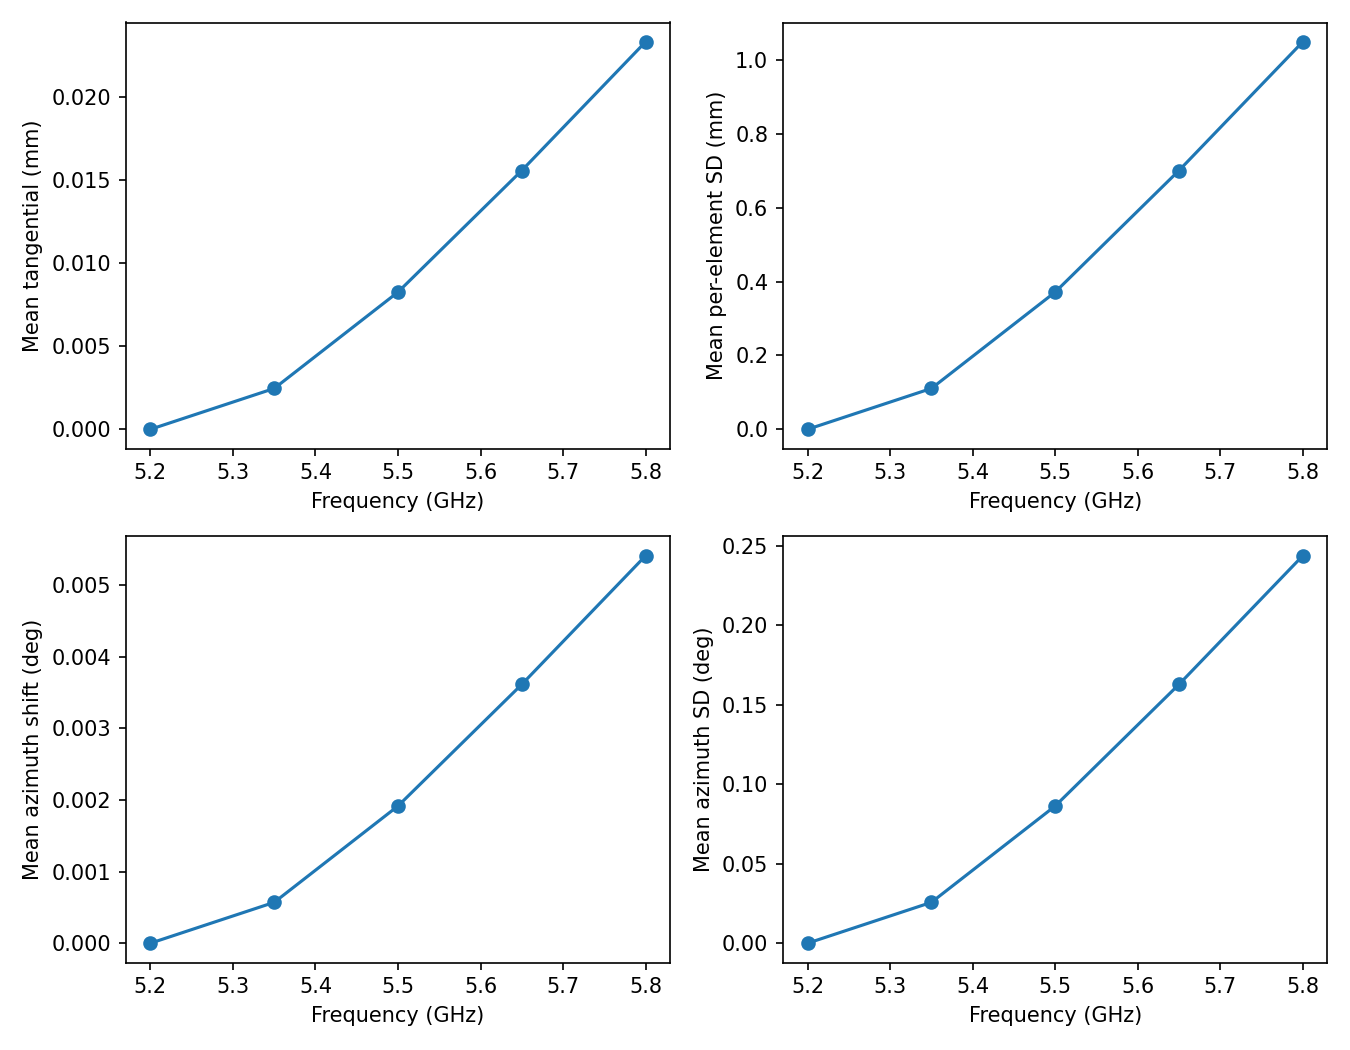
\includegraphics[width=\linewidth]{11_frequency_displacement_statistics.png}\caption{Displacement statistics.}\end{subfigure}\hfill\begin{subfigure}{.48\textwidth}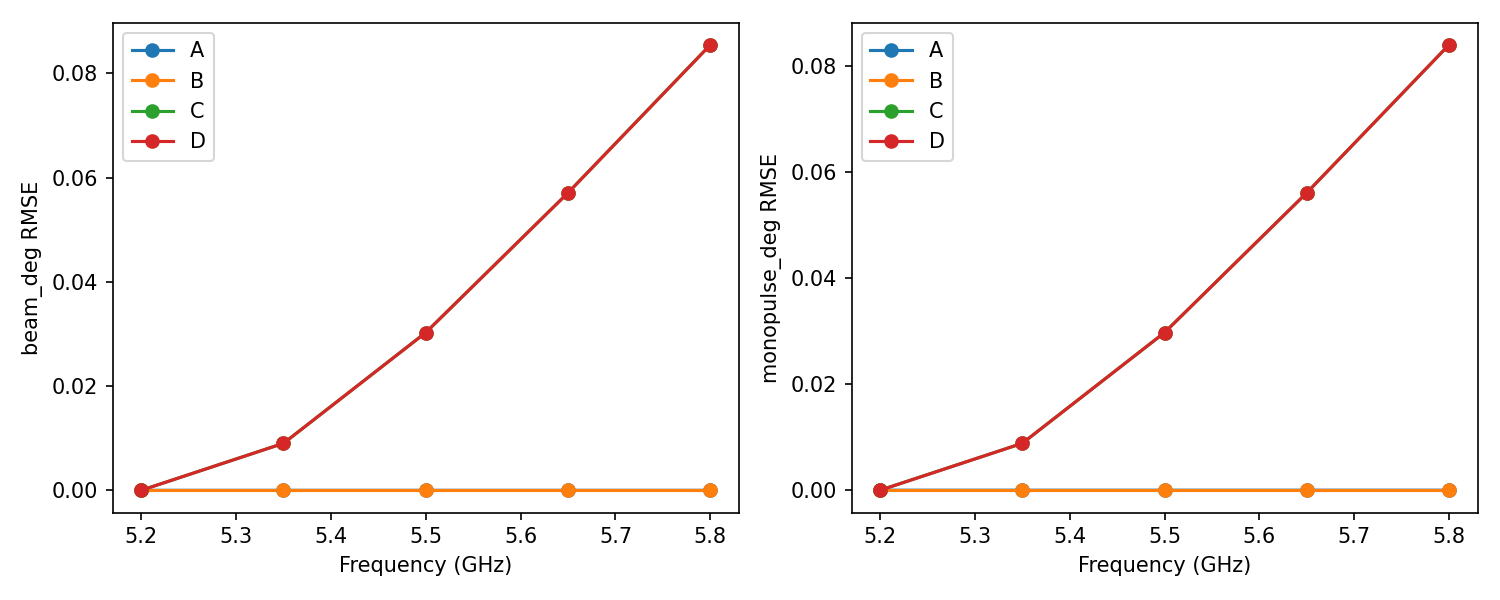
\includegraphics[width=\linewidth]{12_frequency_error_comparison.png}\caption{Error across the band.}\end{subfigure}\caption{Frequency study of the public phase-centre displacement model and error metrics.}\end{figure}

\chapter{Interpretation, limits, and reproducibility}
The project team's assessment was that the modeled error was acceptable for its intended system. Public acceptance criteria are unavailable, so this statement cannot be independently checked from this report. The result supports a modeling conclusion under the selected correlation, displacement magnitude, phase-centre law, weights, target location and calibration. It must not be presented as measured radar accuracy. A complete structural model for validation has not yet been built, and there are no hardware comparisons of mechanical or RF response. The model also omits noise, multipath, coupling and element-normal rotation. Near calibration limits, invalid cases must be inspected alongside conditional RMSE.

The public implementation, exact CSV summaries, and PNG plots are available at \url{https://github.com/houman-akbarzade/radar-array-deformation-analysis}. From its root, install \texttt{python/requirements.txt}, then run \texttt{python python/array\_study.py --mode baseline --trials 500 --validate-generator}, \texttt{--mode frequency}, and \texttt{--mode study} as documented in the repository. The image composition script in \texttt{figures/} recomputes its one example from the Python model and takes the baseline summary CSV as input. This report is a public scientific account of that synthetic implementation; it does not reproduce protected project data or its original numerical configuration.

\appendix
\chapter{Definitions and checks}
The open-arc covariance is positive semidefinite for the exponential kernel used here. The implementation forms a symmetric eigendecomposition, clips only negligible numerical negative eigenvalues, and rejects materially negative values. A 10,000-draw check compares empirical covariance structure with the target element correlation and checks the displacement standard deviation. These checks test code behavior under its own assumptions; physical validation requires separate evidence.

For a small displacement, $e^{jk(\mathbf r+\delta\mathbf r)\cdot\mathbf u}=e^{jk\mathbf r\cdot\mathbf u}e^{jk\delta\mathbf r\cdot\mathbf u}$. Thus the relevant first-order phase change is proportional to projected displacement. Likewise, where the nominal ratio calibration has nonzero local slope $m_0'(\alpha)$, a small ratio perturbation $\delta m$ gives the approximate angular perturbation $\delta\alpha\simeq\delta m/m_0'(\alpha)$. These local relations explain sensitivity; the reported numbers use the full numerical response and calibration inversion.
\end{document}
